\section{Introduction} \label{introduction}
Machine learning techniques are increasingly being used in industrial and scientific applications to gain insight from the data.
Typically, a machine learning pipeline consists of a set of complex data processing steps, chained together, is designed to process a labeled training dataset and results in a machine learning model.
The machine learning model is then used to make predictions on new unlabeled data.
To fully utilize the model,  the model and the pipeline have to be deployed into an environment where they are used to answer prediction queries in real-time.
Typically, feedback in the form of new training data will become available after the model is deployed.
In order to adapt to the new training data and guarantee a high prediction accuracy, new models are constantly trained and re-deployed.
Many platforms, e.g., Velox \cite{crankshaw2014missing}, Clipper \cite{crankshaw2016clipper}, Laser \cite{agarwal2014laser}, and TensorFlow Extended \cite{baylor2017tfx}, provide support for deployment and continuous training of machine learning pipelines. 
These platforms, either automatically or manually, facilitate the training and re-deployment of the models.
In many real-world use cases, training datasets are very large which may require hours of training to obtain a model that guarantees a high quality.
Therefore, it is not feasible to train new models frequently.
This means that the model being used for answering prediction requests is not always up-to-date.
Online learning methods can be utilized to provide fresh and up-to-date models.
However, unless the online learning method is highly tuned to the specific use case, a high-quality model cannot be guaranteed \cite{ma2009identifying}. 
This results in a trade-off between model quality and model freshness.
Addressing the trade-off between quality and freshness is crucial for internet scale applications where both training data and prediction requests are generated with very high speed and large throughput.
One example of internet scale applications is online advertising.
In online advertising, machine learning models are frequently used to provide personalized ads to the users based on their browsing behavior.
\begin{figure}[h!]
\centering
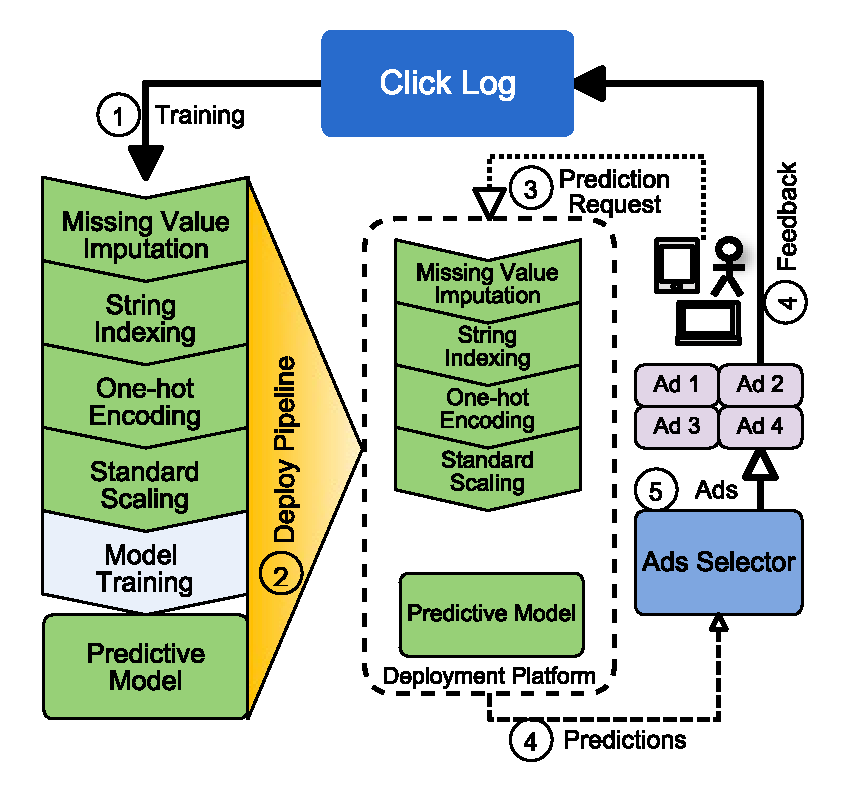
\includegraphics[width=\columnwidth]{../images/motivational-example-vertical.pdf}
\caption{Example Application: Ads Serving}
\label{fig:motivational-example}
\end{figure}

\textbf{Example Application.} 
Online advertising is a multi-billion dollar industry.
An advertising network receives ads from different businesses (ad providers) and shows them on different websites (publishers).
The advertising network charges businesses based on the number of clicks users make on their published ads.
Advertising networks utilize machine learning pipelines to estimate the click rate of different ads.
Figure \ref{fig:motivational-example} shows the workflow of an advertising firm.
The input data (Click Log) consists of several numerical and categorical variables related to the user, the publisher's website, the ads, and whether or not the users clicked on the ads.
A basic click rate prediction pipeline is designed the following way \textcircled{1}. 
A \textbf{missing value imputer} replaces missing values with appropriate values.
A \textbf{string indexer} finds the different unique values in a categorical feature. 
A \textbf{one-hot encoder} creates a new binary feature for every unique value in a categorical feature.
%A \textbf{data bucketizer} transforms continuous variables into a series of binary variables.
A \textbf{standard scaler} scales the data columns to have unit standard deviation and zero mean.
And finally a \textbf{model trainer} trains a logistic regression model over the processed data.
Once the pipeline is created, the deployment platform serves the pipeline and model and prepares them for receiving prediction queries \textcircled{2}.
Whenever a user visits a publisher website, a series of prediction queries are sent to the deployment platform \textcircled{3} .
The deployment platform uses the pipeline to process the request and the model to estimate the click rate of the user for the available ads on the website \textcircled{4}.
An ads selector unit shows the ads with the highest click rate estimates to the user \textcircled{5}.
Depending on whether the user clicks on the ad or not, the platform generates new training data \textcircled{6}.
The deployment platform appends the new training data to the existing click log.
Moreover, new users, ads, and websites may become available while the model is being served.
Therefore, the deployment platform periodically (typically on a daily basis) reprocess the entire data in the click log using the pipeline and trains a new logistic regression model.

The example above demonstrates the complex workflow of a deployment platform.
The deployment platform must be able to guarantee predictions with high accuracy and low latency.
This requires the platform to address the trade-off between the model quality and freshness.
Moreover, the deployment platform must accommodate all the prediction requests and the new training data arriving at the system. 
Our goal is to design a deployment platform that can handle such traffic, provide more accurate predictions to the end user, and provide a balance between model quality and model freshness.

\textbf{Existing Deployment Methods.} 
To ensure accurate predictions, new models should be trained frequently.
However, existing solutions recognize training new models as a resource-intensive and time-consuming process \cite{crankshaw2014missing, agarwal2014laser, baylor2017tfx}.
To address the trade-off between model quality and model freshness, existing solutions propose periodical training of new models.
However, the periods between each instance of the training are typically long (e.g., daily).
While daily training is appropriate for some use cases, it is not suitable for use cases that are required to react quickly to changes in the data (e.g., credit card fraud detection).
This leads to high quality but out-dated models that do not consider the recent training data when answering predictions.
Moreover, existing solutions treat the model training and model serving as two separate processes. 
New models are fully trained in isolation then they are pushed to the deployment environment.

By merging these two processes (training and serving), the training process of new models can be optimized.
In this paper, we propose a method for a deployment platform that continuously updates the models (thus providing fresh models) without sacrificing the quality.
Our solution offers two key optimizations.

\textit{Proactive training.}
Stochastic Gradient Descent (SGD) is an iterative optimization algorithm that is commonly used for training machine learning models on large datasets.
We use SGD to continuously update the deployed model.
Individual iterations of SGD are independent and typically lightweight.
By exploiting these two features of SGD, we replace the time-consuming and resource-intensive training of the new model by a series of single iterations of SGD that are executed proactively.
Our strategy in continuously updating the model is similar to how parameter servers train large models \cite{li2014scaling}.
Parameter servers use the Stochastic Gradient Descent optimization method to iteratively compute partial updates and push these updates to the model.
In our solution, we continuously compute the partial updates based on a combination of the existing data and the newly arrived data.
We then propagate the partial updates to the deployed model.
Proactive training increases model freshness without sacrificing the model quality.
Our experiments show that proactive training of the model achieves more accurate predictions over time and requires fewer resources when compared to the full training of new models.

\textit{Online Statistics Computation and Data Materialization}
We compute and update the statistics of the training dataset in real-time while the model is being served. 
The statistics are required to process the data before training the model.
In our motivating example, label indexing, one-hot encoding, 
%data bucketing, 
and standard scaling require statistics in form of the mean, standard deviation, and feature distribution.
Due to the size of the training dataset, computing these statistics every time before training the model is time-consuming which increases the total training time of the new model.
Updating the statistics in real-time requires a minimal amount of resources. 
To compute mean and standard deviation, we need to update the column sum and dataset size.
To index the labels and perform one-hot encoding, we need to perform a lookup (and in case a new categorical variable is detected, an update) in a hash-table. 
After updating the statistics, each pipeline component transforms the data and passes the data to the next component.
When every component updates their statistics the resulting data is materialized and stored on disk.
As a result, we can directly use the materialized data to train a new model and skip the preprocessing steps of the pipeline.

In summary our contributions are:
\begin{itemize}
\item A platform for continuously training deployed machine learning pipelines and models that adapts to the rate of the incoming data and the model quality requirement.
\item Proactive training of the deployed model using a parameter server style approach that frequently updates the model in-place and increases the quality of the model when compared with state of the art.
\item Efficient training of the model by online statistics computation and data materialization, thus guaranteeing the model freshness without sacrificing the model quality.
\end{itemize}

The rest of this paper is organized as follows:
Section \ref{continuous-training-serving} describes the details of our continuous training approach.
In Section \ref{sec:system-architecture}, we introduce the architecture of our deployment system.
In Section \ref{evaluation}, we evaluate the performance of our continuous deployment approach.
Section \ref {related-work} discusses the related work.
Finally, Section \ref{conclusion} presents our conclusion and the future work.
